\documentclass[aspectratio=169]{beamer}

% =========================================================
% THEME
% =========================================================

\usetheme{metropolis}

% =========================================================
% PACKAGES
% =========================================================

\usepackage{booktabs}
\usepackage{graphicx}
\usepackage{amsmath}
\usepackage{multirow}
\usepackage{animate}
\usepackage{tabularray}
\usepackage{tabularx}
\usepackage{arydshln}
\usepackage[authoryear,round]{natbib}
\usepackage{tikz}
\usetikzlibrary{arrows.meta, positioning, shapes.geometric}
\usepackage{pgfplots}
\usepackage{appendixnumberbeamer}
\usepackage[most]{tcolorbox}
\usepackage{csquotes}
\usepackage{setspace}

\pgfplotsset{compat=1.18}
\setcitestyle{authoryear,round,aysep={, }}

% =========================================================
% COLORS
% =========================================================

\definecolor{SpaceBlue}{RGB}{15,25,45}
\definecolor{SpaceCyan}{RGB}{0,180,220}
\definecolor{SoftGreen}{RGB}{228,244,235}
\definecolor{SoftOrange}{RGB}{255,242,225}
\definecolor{SoftBlue}{RGB}{230,240,255}

\setbeamercolor{frametitle}{bg=SpaceBlue, fg=white}
\setbeamercolor{title separator}{fg=SpaceCyan}
\setbeamercolor{progress bar}{fg=SpaceCyan}
\setbeamercolor{alerted text}{fg=SpaceBlue}
\hypersetup{
    colorlinks=true,
    citecolor=SpaceBlue,
    linkcolor=SpaceBlue,
    urlcolor=SpaceBlue
}

\setbeamertemplate{itemize item}{\textbullet}
\setbeamertemplate{itemize subitem}{--}

\newcommand{\BaselineAnim}[2][0.47\linewidth]{%
  \animategraphics[autoplay,loop,width=#1,trim={2cm 3.4cm 3.1cm 1.5cm},clip]{8}{figures/baselines/#2/frame}{0}{101}%
}

\newcommand{\myCustomSize}[1]{%
  \fontsize{5}{6}\selectfont
  #1
}

\newcommand{\probP}{\text{I\kern-0.15em P}}

\newcommand{\ComparisonAnimations}[2]{%
  \begin{columns}[T,totalwidth=\textwidth]
    \begin{column}{0.49\textwidth}
      \centering
      {\footnotesize\textbf{Reference: ORBITAL-MOISE+MARL}}\\[-0.05cm]
      \BaselineAnim[0.92\linewidth]{ORBITAL-MOISE+MARL}
    \end{column}
    \begin{column}{0.49\textwidth}
      \centering
      {\footnotesize\textbf{#2}}\\[-0.01cm]
      \BaselineAnim[0.92\linewidth]{#1}
    \end{column}
  \end{columns}
}

\newcommand{\CompactItem}[1]{\item \scriptsize #1}

\newcommand{\ExplainerImage}[2][0.92\linewidth]{%
  \includegraphics[width=#1]{figures/explainer/#2}%
}

% =========================================================
% TITLE
% =========================================================

\title{
Toward Automated Operational Assist \\
in Satellite Fleet Management \\
via Organizational MARL
}

\author{\textbf{Julien Soulé}}

\institute{
SEDAN Research Group -- SnT \\
University of Luxembourg
}

\logo{
    
\includegraphics[width=0.16\textwidth]{figures/snt_logo.jpg}
}

\date{
MASSpace @ AAMAS 2026 \\
May 26, 2026
}

% =========================================================
% BEGIN DOCUMENT
% =========================================================

\begin{document}

{
\setbeamertemplate{footline}{}
\begin{frame}
  \titlepage
\end{frame}
}

\setcounter{framenumber}{0}

\logo{}

\begin{frame}{An increasingly difficult satellite-fleet monitoring problem}

  \begin{columns}[c,totalwidth=\textwidth]
    \begin{column}{0.43\textwidth}
      \begin{itemize}
        \item Dynamic observation demand
        \item Short communication windows
        \item Limited energy and buffer capacity
        \item Cyber and jamming events
        \item Debris and collision-risk pressure
      \end{itemize}

      \vspace{0.2cm} \ \\
      \textbf{Automated support with controllability and explainability for partial assistance?}
    \end{column}
    \begin{column}{0.55\textwidth}
      \centering
      \animategraphics[autoplay,loop,width=\linewidth,height=0.58\textheight,keepaspectratio]{8}{figures/3d_illustration_render/frame}{0}{239}\\[0.2cm]
      {\scriptsize\linespread{0.82}\selectfont Illustrative view of cooperative satellites operating under task, relay, and safety pressure.\par}
    \end{column}
  \end{columns}

\end{frame}

\begin{frame}{Related works and gaps}

  \scriptsize
  \setlength{\tabcolsep}{4pt}
  \renewcommand{\arraystretch}{1.5}
  \begin{tabularx}{\linewidth}{p{4.05cm}|X X}
    \toprule
    Family & Strengths                                                                        & Gaps \\
    \midrule
    (A) Satellite planning, scheduling, digital twins
           & operational constraints; optimized plans; domain realism
           & few reusable decentralized-learning and audit benchmarks                                \\
    \hdashline
    (B) DCOP and planning
           & explicit constraints; coordination; guarantees
           & adaptation remains difficult under partial observability and disturbances               \\
    \hdashline
    (C) Dec-POMDP, MARL
           & decentralized learning; adaptation
           & controllability and XRL are often left to external methods                              \\
    \hdashline
    (D) \textbf{Constrained/Guided MARL}
           & norms, convergence, stability, XRL/XMARL
           & \textbf{promising fit, but no satellite-fleet simulator and ready-to-use models}        \\
    \bottomrule
  \end{tabularx}

  \vspace{0.16cm}
  {\tiny
    A: \citep{ferrari2025ssp_survey,rocha2025iaeossp,govoni2026multi_sat_task_allocation}. B: \citep{Krigman2024,hoang2022proactive}. C: \citep{Oliehoek2016,rashid2018qmix,yu2021mappo}. (D) \textbf{\citep{ferber2003,Hubner2002,Hubner2007,puiutta2020xrlsurvey,soule2024moise_marl,garcia2015comprehensive,alshiekh2018safe}}.\par
  }

\end{frame}

\begin{frame}{Hypotheses and contributions}

  \begin{tcolorbox}[
      colback=white,
      colframe=blue!60!black,
      boxrule=0.8pt,
      arc=1mm,
      left=2mm,
      right=2mm,
      top=1mm,
      bottom=1mm
    ]

    Organizational MARL approach for Earth-observation satellite-fleet management
    \begin{itemize}
      \item agents automatically coordinate under environmental constraints.
      \item inject prior knowledge into MARL $\rightleftarrows$ extract posterior organizational insights
    \end{itemize}

  \end{tcolorbox}


  \vspace{1cm}

  We propose:
  \begin{itemize}
    \item A controlled benchmark for fleet-level operational-assist experiments.
    \item An adapted organizational MARL framework with roles and goals for prior knowledge injection and post-hoc analysis.
  \end{itemize}

\end{frame}

\begin{frame}{Orbital Resilient Benchmark for
    Interactive Task-aware Autonomous Learning}

  \vspace{0.1cm}
  \begin{columns}[c,totalwidth=\textwidth]

    \begin{column}{0.\textwidth}
    \end{column}

    \hspace{-1cm}
    \begin{column}{0.6\textwidth}
      \tiny

      % \animategraphics[autoplay,loop,width=\linewidth,trim={2cm 3.4cm 3.1cm 1.5cm},clip]{8}{figures/2d_illustration_render/frame}{0}{299}

      \animategraphics[autoplay,loop,width=\linewidth,trim={2cm 3.4cm 3.1cm 1.5cm},clip]{8}{figures/2d_illustration_render/frame}{0}{239}

      View of ORBITAL: each satellite is an agent, receives observations and makes decisions to support acquisition (go toward \textit{observation tasks}); delivery (relay to \textit{ground stations}); and stabilization (handle \textit{health}, \textit{energy}, \textit{cyber}, \textit{isolation}). Health decreases due to debris collisions or when satellites are randomly compromised by cyber events. Energy is consumed by actions and can be recovered by low-power mode. Communication is intermittent and can be jammed.
    \end{column}

    \begin{column}{0.4\textwidth}
      \myCustomSize
      \textbf{Observation space.} 20-dimensional local state.
      \renewcommand{\arraystretch}{1.2}
      \begin{tabularx}{1.2\linewidth}{p{1.3cm} X}
        \toprule
        Family           & Features                                                       \\
        \midrule
        State and orbit  & energy, health, $\theta$, radius, $\phi$, sunlight             \\
        Communication    & direct ground contact, network route, local degree, jamming    \\
        Data and tasks   & buffer load, remaining capacity, task and priority             \\
        Safety and cyber & debris density, collision risk, compromised state, recent scan \\
        Fleet context    & compromised-neighbor ratio and alive-satellite fraction        \\
        \bottomrule
      \end{tabularx}

      \vspace{0.4cm}
      \textbf{Action space.} Scalar action between 0 and 7.
      \begin{tabularx}{1.2\linewidth}{p{1.09cm} X}
        \toprule
        Action                  & Main effect                                                             \\
        \midrule
        \texttt{observe}        & services a local task and fills the buffer (energy $\downarrow$)        \\
        \texttt{relay\_ground}  & delivers data and syncs task knowledge via ground (energy $\downarrow$) \\
        \texttt{relay\_sat}     & shares knowledge or transfers data to a neighbor (energy $\downarrow$)  \\
        \texttt{orbit\_down/up} & changes radius, connectivity, and debris exposure (energy $\downarrow$) \\
        \texttt{lowpower}       & reduces consumption and can recover energy                              \\
        \texttt{cyberscan}      & mitigates compromise risk (energy $\downarrow$)                         \\
        \texttt{idle}           & waits while orbital dynamics continue                                   \\
        \bottomrule
      \end{tabularx}
    \end{column}
    \vspace{-0.5cm}
  \end{columns}

\end{frame}



\begin{frame}{Acquire, deliver, stabilize}

  \vspace{0.1cm}
  \begin{columns}[c,totalwidth=\textwidth]

    \begin{column}{0.5\textwidth}

      \scriptsize

      \textbf{Operational tension}

      \begin{itemize}
        \item Acquire
              \begin{itemize}
                \item {\scriptsize useful only if the data can later be delivered;}
                \item {\scriptsize limited by task knowledge, position, energy, and buffer.}
              \end{itemize}

        \item Deliver
              \begin{itemize}
                \item {\scriptsize high value through ground contact;}
                \item {\scriptsize depends on relay paths and timing.}
              \end{itemize}

        \item Stabilize
              \begin{itemize}
                \item {\scriptsize protects energy, health, cyber state, and debris safety;}
                \item {\scriptsize often delays acquisition or delivery.}
              \end{itemize}
      \end{itemize}

    \end{column}

    \begin{column}{0.01\textwidth}
    \end{column}

    \begin{column}{0.5\textwidth}

      \myCustomSize

      \vspace{0.05cm}
      \renewcommand{\arraystretch}{1.5}
      \begin{tabularx}{\linewidth}{p{3cm}p{.8cm} X}
        \toprule

        Reward rule & Component                               & Reward effect \\
        \midrule

        Ground relay with buffered data and valid contact
                    & delivery
                    & $+1000 \times$ delivered data                           \\

        Observe active, known, reachable task
                    & task
                    & $+100 \times$ observed data                             \\

        Task knowledge discovered or shared
                    & knowledge
                    & $+10 \times$ knowledge gain                             \\

        Ground contact imports catalog tasks
                    & intake
                    & $+1 \times$ new tasks                                   \\

        Any action consumes energy
                    & energy
                    & $-0.05 \times$ energy spent                             \\

        Observation exceeds buffer capacity
                    & overflow
                    & $-0.4 \times$ lost data                                 \\

        Destroyed satellite loses buffered data
                    & data loss
                    & $-0.8 \times$ lost data                                 \\

        Malware, drag, or collision reduces health
                    & health
                    & $-0.8 \times$ health loss                               \\

        Living satellite has no communication neighbor
                    & isolation
                    & $-0.3 \times$ isolated satellites                       \\

        Dead satellites remain in the fleet
                    & failure
                    & $-1.0 \times$ dead satellites                           \\

        Compromise, jamming, forced action, drag, debris, collision
                    & safety costs
                    & $-0.4$ to $-2.5 \times$ event intensity                 \\

        \bottomrule
      \end{tabularx}

    \end{column}
    \vspace{-0.5cm}
  \end{columns}

\end{frame}


\begin{frame}{$\mathcal{M}OISE^+$ and MOISE+MARL}

  \vspace{0.3cm}

  \begin{columns}[c,totalwidth=\textwidth]
    \scriptsize
    \hspace{-0.5cm}
    \begin{column}{0.40\textwidth}
      \scriptsize
      $\mathcal{M}OISE^+$~\citep{Hubner2002,Hubner2007} is a highly formalized organizational model
      \begin{itemize}
        \item structural (roles),
        \item functional (goals);
        \item and deontic (permissions/obligations)
      \end{itemize}

      \vspace{0.5cm}

      Decentralized Partially Observable Markov Decision Process (Dec-POMDP) \citep{Oliehoek2016}
      \begin{itemize}
        \item considers multiple agents in a MAS-like setting
        \item stochastic processes for uncertainty in environmental changes including observations;
        \item $(S,\{A_i\},T,R,\{\Omega_i\},O,\gamma)$
      \end{itemize}

    \end{column}

    \begin{column}{0.04\textwidth}
    \end{column}

    \begin{column}{0.65\textwidth}
      \scriptsize
      MOISE+MARL~\citep{soule2024moise_marl} binds $\mathcal{M}OISE^+$ and MARL
      \begin{itemize}
        \setlength{\itemsep}{2pt}
        \setlength{\parskip}{0pt}
        \setlength{\parsep}{0pt}

        \item \scriptsize \textbf{Roles provide shielding}
              \begin{itemize}
                \setlength{\itemsep}{0pt}
                \item \scriptsize input: current observation;
                \item \scriptsize output: actions allowed at this step;
                \item \scriptsize effect: replace forbidden policy actions by allowed ones.
              \end{itemize}

        \item \scriptsize \textbf{Goals provide reward shaping}
              \begin{itemize}
                \setlength{\itemsep}{0pt}
                \item \scriptsize input: history, current observation, selected action;
                \item \scriptsize output: bonus or malus added to the reward;
                \item \scriptsize effect: guide learning toward intermediate objectives.
              \end{itemize}

        \item \scriptsize \textbf{Trajectory-based Evaluation in MOISE+MARL (TEMM) provides organizational analysis}
              \begin{itemize}
                \setlength{\itemsep}{0pt}
                \item \scriptsize input: trajectories;
                \item \scriptsize output: structural, functional, and organizational fit scores;
                \item \scriptsize effect: post-hoc evidence of organizational traces (org. fit).
              \end{itemize}
      \end{itemize}
    \end{column}
  \end{columns}

\end{frame}

\begin{frame}{ORBITAL-oriented MOISE+MARL}

  \tiny
  \setlength{\tabcolsep}{3.5pt}
  \renewcommand{\arraystretch}{1.08}
  \begin{tabularx}{\linewidth}{p{2.25cm} X X}
    \toprule
    Element & Rule sketch                                                                                                                 & Effect \\
    \midrule
    \texttt{acquirer} role
            & use \texttt{relay\_ground} to obtain the task catalog; use \texttt{observe} when a known nearby task and buffer space exist
            & turns ground catalog access into useful task acquisition                                                                             \\
    \texttt{deliverer} role
            & use \texttt{relay\_ground} for buffered data; use \texttt{relay\_sat} when a route or neighbor can help
            & moves buffered mission data and task knowledge toward delivery                                                                       \\
    \texttt{stabilizer} role
            & use \texttt{scan}, \texttt{lowpower}, or orbit actions under cyber, energy, jamming, or debris stress
            & preserves future action capacity and reduces mission collapse                                                                        \\
    \texttt{acquirer\_goal}
            & bonus actions that match the acquirer logic; small malus when a relevant acquisition action is ignored
            & makes catalog intake and observation easier to learn                                                                                 \\
    \texttt{deliverer\_goal}
            & bonus actions that match the deliverer logic; small malus when a relevant delivery action is ignored
            & links local relay decisions to final mission value                                                                                   \\
    \texttt{stabilizer\_goal}
            & bonus actions that match the stabilizer logic; small malus when a relevant safety action is ignored
            & encourages recovery from cyber, energy, and debris stress                                                                            \\
    \bottomrule
  \end{tabularx}

  \vspace{0.12cm}
  \small
  Partial roles impose their handcrafted action with constraint hardness $0.3$; full roles impose it with hardness $1.0$.

\end{frame}

\begin{frame}{Baselines}

  \tiny
  \vfill
  \begin{center}
    \setlength{\tabcolsep}{3pt}
    \renewcommand{\arraystretch}{1.3}
    \begin{tabularx}{0.96\linewidth}{p{2.55cm} p{2.85cm} X}
      \toprule
      Family & Condition                                                                                               & What it tests \\
      \midrule
      Rule-Based
             & \texttt{handcrafted}
             & A fully scripted acquire--deliver--stabilize loop; interpretable operational control without learning.                  \\
      Rule-Based
             & \texttt{rb\_deliverer}
             & Delivery continuity first: full \texttt{deliverer}, with softer acquisition and stabilization.                          \\
      Rule-Based
             & \texttt{rb\_dcop\_like}
             & DCOP-inspired structure: full \texttt{acquirer} and \texttt{deliverer}, soft \texttt{stabilizer}.                       \\
      Rule-Based
             & \texttt{rb\_acquirer}
             & Acquisition-first control: full \texttt{acquirer}, with softer delivery and stabilization.                              \\
      Learning-Based
             & \texttt{lb\_unconstrained}
             & Same MARL backbone with the native ORBITAL reward only; tests adaptation without explicit organization.                 \\
      Learning-Based
             & \texttt{lb\_reward\_only}
             & Goal-reward guidance only; isolates whether shaping can induce mission discipline without shielding.                    \\
      Learning-Based
             & \texttt{lb\_action\_only}
             & Role-action shielding only; isolates structural control without extra mission rewards.                                  \\
      \bottomrule
    \end{tabularx}

    \vspace{0.16cm}
    \small
    The comparison separates interpretable rule-based control from adaptive learning-based ablations.
  \end{center}
  \vfill

\end{frame}

\begin{frame}{Experimental setup}

  \scriptsize
  \begin{columns}[c,totalwidth=\textwidth]
    \hspace{-0.5cm}
    \begin{column}{0.45\textwidth}
      \scriptsize
      \textbf{Software}

      \begin{itemize}
        \item ORBITAL\footnote{\scriptsize\url{https://github.com/julien6/ORBITAL}} is a PettingZoo environment\citep{terry2020pettingzoo}
        \item The MOISE+MARL framework and baselines\footnote{\scriptsize\url{https://github.com/julien6/BenchMARL}} are implemented within BenchMARL\citep{bettini2024benchmarl}
      \end{itemize}


      \vspace{0.25cm}
      \textbf{Hardware (NVIDIA DGX Spark Version 7.4.0)}
      \begin{tabularx}{\linewidth}{p{1cm} X}
        \toprule
        CPU & 20 physical/logical cores at 3354 MHz \\
        RAM & 119.69 GB total                       \\
        GPU & NVIDIA GB10, 48 SMs, 119.69 GB VRAM   \\
        \bottomrule
      \end{tabularx}
    \end{column}
    \begin{column}{0.55\textwidth}
      \textbf{Hyperparameters}
      \begin{tabularx}{\linewidth}{p{1.2cm} X}
        \toprule
        Selection & HPO with BenchMARL sweeps on validation seeds
          {\tiny
        \begin{itemize}
              \item \tiny MAPPO~\citep{yu2021mappo}, QMIX~\citep{rashid2018qmix}, MASSAC~\citep{pu2021decomposedsoftactorcriticmethod}
            \end{itemize}} \\[-0.3cm]
        Budget    & same episode horizon and optimization budget across learning conditions                                     \\
        Seeds     & disjoint training, selection, and final-evaluation seeds                                                    \\
        \bottomrule
      \end{tabularx}

      \vspace{0.32cm}
      \textbf{Metrics}
      \begin{tabularx}{\linewidth}{p{1.2cm} X}
        \toprule
        Mission    & return, delivery volume, and mission success           \\
        Robustness & energy stress, isolation, failures, cyber impact       \\
        Control    & role-violation rate and consistency indicators         \\
        Audit      & structural fit, functional fit, and organizational fit \\
        \bottomrule
      \end{tabularx}
    \end{column}
  \end{columns}

\end{frame}


\begin{frame}{Results overview}

  \scriptsize
  \vfill
  \begin{center}
    \setlength{\tabcolsep}{5pt}
    \renewcommand{\arraystretch}{1.03}
    Metric values normalized over experimental values across all baselines for MAPPO\citep{yu2021mappo}
    \begin{tabularx}{0.99\linewidth}{c c c c c c c}
      \toprule
      Condition                  & Final return    & Std. dev.       & Robustness      & Convergence     & Rule violation  & OF score        \\
      \midrule
      \texttt{handcrafted}       & $0.82$          & $0.04$          & $0.47$          & n/a             & n/a             & n/a             \\
      \texttt{rb\_deliverer}     & $0.67$          & $0.04$          & $0.50$          & n/a             & n/a             & n/a             \\
      \texttt{rb\_dcop\_like}    & $0.60$          & $0.05$          & $0.53$          & n/a             & n/a             & n/a             \\
      \texttt{rb\_acquirer}      & $0.64$          & $0.04$          & $0.45$          & n/a             & n/a             & n/a             \\
      \texttt{lb\_unconstrained} & $\mathbf{0.95}$ & $0.17$          & $\mathbf{0.86}$ & $0.50$          & $0.74$          & $0.52$          \\
      \texttt{lb\_reward\_only}  & $0.90$          & $0.15$          & $0.85$          & $0.58$          & $0.63$          & $0.67$          \\
      \texttt{lb\_action\_only}  & $0.83$          & $0.12$          & $0.77$          & $0.68$          & $0.31$          & $0.79$          \\
      \texttt{lb\_moise\_marl}   & $0.85$          & $\mathbf{0.08}$ & $0.80$          & $\mathbf{0.70}$ & $\mathbf{0.18}$ & $\mathbf{0.91}$ \\
      \bottomrule
    \end{tabularx}

    \vspace{0.45cm}
    \small
    Finding a trade-off between constraining too much (rule-based) and constraining too little (unconstrained learning).
  \end{center}
  \vfill

\end{frame}

\begin{frame}{Full MOISE+MARL vs LB-Unconstrained}
  \ComparisonAnimations{LB-Unconstrained}{LB-Unconstrained}
  \vspace{-0.5cm}
  \begin{block}
    \scriptsize
    \begin{itemize}
      \item{\scriptsize LB-Unconstrained uses the same MARL backbone without organizational roles or goals.}
      \item{\scriptsize Full MOISE+MARL appears easier to audit when communication, energy, and cyber pressure interact.}
    \end{itemize}
  \end{block}
  \vspace{0.15cm}
  \tiny
  \textit{Training, evaluation, and TEMM traces are summarized in Wandb: \url{https://wandb.ai/julien-soule-university-of-luxembourg/benchmarl?nw=nwuserjuliensoule}.}
\end{frame}

\begin{frame}{Conclusion, limits, and perspectives}

  \small
  \begin{itemize}
    \item Proposed the \textbf{ORBITAL benchmark} for satellite-fleet operational-assist research.
    \item Developed an \textbf{organizational MARL framework} for satellite-fleet guidance and analysis.
    \item Organizational priors can improve performance quickly with explainability and control.
  \end{itemize}

  \vspace{0.2cm}
  \textbf{Limits and future work}
  \begin{itemize}
    \item Organizational priors can improve auditability, but overly rigid roles may reduce adaptation (trade-off).
    \item ORBITAL remains an abstraction of orbital mechanics, communication, and operational procedure.
    \item The framework has computational overhead because several baselines, sweeps, and trajectory analyses are needed.
    \item TEMM still requires careful audit, semantic interpretation, and manual intervention.
  \end{itemize}

\end{frame}

\logo{
  
\includegraphics[width=0.16\textwidth]{figures/snt_logo.jpg}
}

\setbeamertemplate{footline}{}

\begin{frame}
  \centering
  \vspace{1cm}
  {\Huge Thank You}\\
  \vspace{1cm}
  {\Large Questions?}\\
  \vspace{2.3cm}
  \textit{julien.soule@uni.lu}
\end{frame}

\logo{}

\begin{frame}[allowframebreaks]{References}
  \scriptsize
  \bibliographystyle{ACM-Reference-Format}
  \bibliography{references}
\end{frame}

% =========================================================
% APPENDIX
% =========================================================

\appendix


\begin{frame}{Training}{Standard MARL}

  \begin{itemize}
    \item Select the best actions to maximize cumulative reward
  \end{itemize}

  \begin{center}
    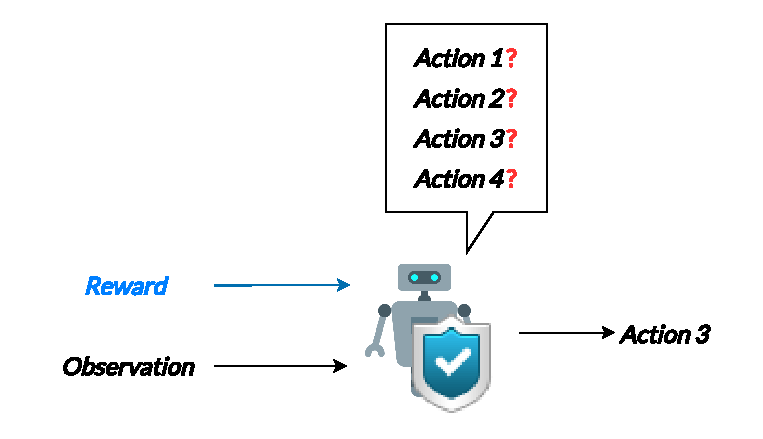
\includegraphics[width=0.5\linewidth]{figures/vanilla_marl.pdf}
  \end{center}

\end{frame}

\begin{frame}{Training}{Guided / Constrained Learning}

  \textbf{MARL + organization}
  \begin{itemize}
    \item Role: enforce / forbid actions $\rightarrow$ safety guarantee
  \end{itemize}

  \begin{center}
    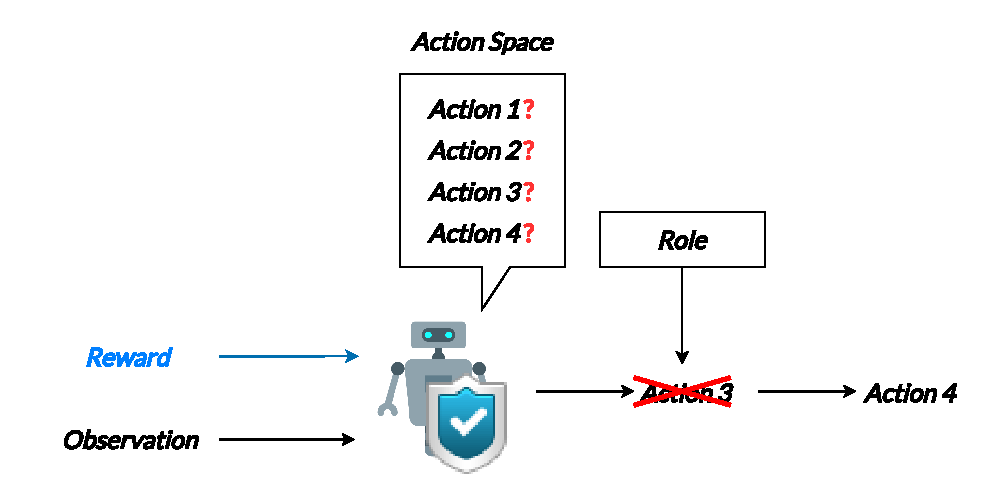
\includegraphics[width=0.5\linewidth]{figures/role_marl.pdf}
  \end{center}

\end{frame}

\begin{frame}{Training}{Guided / Constrained Learning}

  \textbf{MARL + organization}
  \begin{itemize}
    \item Goal: encourage the achievement of an intermediate objective
  \end{itemize}

  \begin{center}
    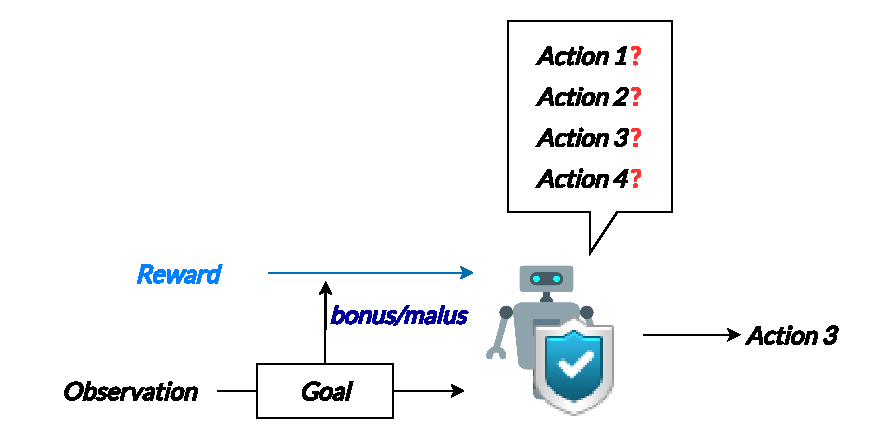
\includegraphics[width=0.5\linewidth]{figures/goal_marl.pdf}
  \end{center}

\end{frame}

\begin{frame}{Training}{The MOISE+MARL Framework}

  \begin{columns}[c] % c = vertically center content
    \begin{column}{0.5\textwidth}
      \begin{itemize}
        \item Combine Dec-POMDP with $\mathcal{M}OISE^+$.
        \item Agents $\rightarrow$ role and mission $\rightarrow$ goals.
        \item Constraint guides $\sim$ \textquote{role / goal implementation}:
              \begin{itemize}
                \item \textbf{Actions} via \textit{RoleActionGuides} (RAG)
                \item \textbf{Rewards} via \textit{RoleRewardGuides} and \textit{GoalRewardGuides}
              \end{itemize}
      \end{itemize}
    \end{column}
    \begin{column}{0.6\textwidth}
      \begin{figure}
        \centering

        \vspace{0.1cm}

        \resizebox{1\linewidth}{!}{
          \input{figures/mm_synthesis_single_column.tex}
        }


      \end{figure}
    \end{column}
  \end{columns}

\end{frame}

\begin{frame}{Analysis}{Method Overview}

  \footnotesize

  \textbf{Trajectory-based Evaluation in MOISE+MARL (TEMM)}
  \begin{itemize}
    \item \textbf{Objective}: provide a post-hoc interpretation of agent behavior at the organizational level.
    \item \textbf{Hypothesis}: trajectories are ``noisy'' variants of a limited number of strategies.

  \end{itemize}

  \vspace{0em}
  \textbf{Underlying hypotheses:}
  \begin{itemize}
    \item \textbf{Roles} correspond to frequent \emph{(observation, action)} transition patterns in agent trajectories.
    \item \textbf{Goals} correspond to observations frequently received within agent trajectories.
  \end{itemize}

  \vspace{0.1cm}
  \begin{center}
    \begin{columns}[c]

      \begin{column}{0.4\textwidth}
        \centering
        \input{figures/abstract_obs_processed_viz.tex}
      \end{column}

      \begin{column}{0.1\textwidth}
      \end{column}

      \begin{column}{0.4\textwidth}
        \centering
        \input{figures/abstract_full_processed_viz.tex}
      \end{column}
    \end{columns}
  \end{center}

  \begin{tikzpicture}[remember picture, overlay]
    \node[anchor=north west, text=black]
    at ([xshift=5.7cm,yshift=-5.2cm]current page.north west) {\small
      \begin{minipage}{0.3\linewidth}
        {\footnotesize \hspace{0.cm} \textit{\textbf{Operationalization\dots}}
          \begin{itemize}
            \item  \textit{Trajectories as vectors;}
            \item  \textit{Distances: Smith-Waterman, LCS, Euclidean\dots;}
            \item  \textit{Clustering + centroids \\ \ \ \ $\rightarrow$ roles / goals}
          \end{itemize}}
      \end{minipage}

    };
  \end{tikzpicture}

\end{frame}


\begin{frame}{ORBITAL Encodes the Operational Couplings}

  \begin{columns}[T]
    \column{0.52\textwidth}
    \small
    \textbf{Modeled pressures}
    \begin{itemize}
      \item non-stationary prioritized tasks;
      \item finite energy and heterogeneous action costs;
      \item stochastic communication degradation;
      \item stochastic compromise events;
      \item drifting debris-risk zones.
    \end{itemize}

    \vspace{0.2cm}
    \textbf{Core doctrine}
    \begin{center}
      \large Acquire $\rightarrow$ Deliver $\rightarrow$ Stabilize
    \end{center}

    \column{0.48\textwidth}
    \small
    \textbf{Experimental value}
    \begin{itemize}
      \item local task service can conflict with fleet delivery;
      \item safety-preserving actions can reduce short-term reward;
      \item robust behavior requires switching between mission phases;
      \item these switches can be evaluated in trajectories.
    \end{itemize}
  \end{columns}

\end{frame}

\begin{frame}{Visual Grammar}
  \scriptsize
  \begin{columns}[T,totalwidth=\textwidth]
    \begin{column}{0.31\textwidth}
      \centering
      \ExplainerImage[0.70\linewidth]{satellite_marker.png}
      \begin{block}{Satellite marker}
        Number = satellite id. Cyan top bar = buffered data. Green bottom bar = energy. Text labels show role and last action.
      \end{block}
    \end{column}
    \begin{column}{0.31\textwidth}
      \centering
      \ExplainerImage[0.70\linewidth]{observation_task.png}
      \begin{block}{Observation task}
        Warm dots are active tasks. Brighter/larger means higher priority. A successful OBS action removes the task and fills a buffer.
      \end{block}
    \end{column}
    \begin{column}{0.31\textwidth}
      \centering
      \ExplainerImage[0.58\linewidth]{mission_panel.png}
      \begin{block}{Mission panel}
        Watch alive satellites, isolated satellites, delivered value, and reward components to understand the global effect.
      \end{block}
    \end{column}
  \end{columns}
\end{frame}

\begin{frame}{Connectivity}
  \scriptsize
  \begin{columns}[T,totalwidth=\textwidth]
    \begin{column}{0.48\textwidth}
      \centering
      \ExplainerImage[0.82\linewidth]{communication_links.png}
      \begin{block}{Blue communication links}
        Blue lines mean satellites can communicate at this step. They are not deliveries by themselves; they are possible relay paths.
      \end{block}
    \end{column}
    \begin{column}{0.48\textwidth}
      \centering
      \ExplainerImage[0.40\linewidth]{ground_downlink.png}
      \begin{block}{Green ground/downlink cue}
        A green square is a ground station. A green downlink line means buffered data currently has a feasible path to ground.
      \end{block}
    \end{column}
  \end{columns}
\end{frame}

\begin{frame}{Labels}
  \scriptsize
  \begin{columns}[T,totalwidth=\textwidth]
    \begin{column}{0.45\textwidth}
      \centering
      \ExplainerImage[0.78\linewidth]{satellite_marker.png}
    \end{column}
    \begin{column}{0.53\textwidth}
      \begin{block}{Role labels}
        \begin{tabularx}{\linewidth}{>{\bfseries}l X}
          OBS  & Observer role: prioritize acquiring task data.                \\
          REL  & Relay role: prioritize delivery and communication utility.    \\
          SAFE & Safety role: preserve energy, cyber health, or debris safety. \\
          FREE & No organizational role constraint.                            \\
          SOFT & Reward-shaped guidance, but no hard role enforcement.         \\
        \end{tabularx}
      \end{block}
      \begin{block}{Action labels}
        \begin{tabularx}{\linewidth}{>{\bfseries}l X}
          OBS      & Observe task.                                        \\
          REL\_GRN & Relay to ground. \quad REL\_SAT: relay to satellite. \\
          PWR      & Low-power safe mode.                                 \\
          SCAN     & Cyber scan. \quad UP/DN: orbit maneuver.             \\
          IDLE     & No active mission operation this step.               \\
        \end{tabularx}
      \end{block}
    \end{column}
  \end{columns}
\end{frame}

\begin{frame}{Action Transition -- Observe}
  \scriptsize
  \begin{columns}[T,totalwidth=\textwidth]
    \begin{column}{0.33\textwidth}
      \centering
      \ExplainerImage[0.70\linewidth]{observation_task.png}
      \begin{block}{Before}
        A nearby active task is visible as a warm dot. The satellite must be close enough to sense it.
      \end{block}
    \end{column}
    \begin{column}{0.30\textwidth}
      \begin{block}{Action}
        \textbf{OBS}: the satellite spends energy to service one local task.
      \end{block}
      \begin{block}{Immediate effect}
        The task becomes inactive and the satellite's cyan buffer increases.
      \end{block}
    \end{column}
    \begin{column}{0.33\textwidth}
      \centering
      \ExplainerImage[0.78\linewidth]{satellite_marker.png}
      \begin{block}{After}
        The data is only stored. Delivery still requires relay plus a path to ground.
      \end{block}
    \end{column}
  \end{columns}
\end{frame}

\begin{frame}{Action Transition -- Relay}
  \scriptsize
  \begin{columns}[T,totalwidth=\textwidth]
    \begin{column}{0.34\textwidth}
      \centering
      \ExplainerImage[0.70\linewidth]{satellite_marker.png}
      \begin{block}{Before}
        A satellite has buffered data: cyan bar above the marker.
      \end{block}
    \end{column}
    \begin{column}{0.30\textwidth}
      \begin{block}{Actions}
        \textbf{REL\_GRN}: deliver to ground.\\
        \textbf{REL\_SAT}: relay to another satellite.
      \end{block}
      \begin{block}{Requirement}
        Delivery succeeds only with direct ground contact or a communication path through other satellites.
      \end{block}
    \end{column}
    \begin{column}{0.32\textwidth}
      \centering
      \ExplainerImage[0.48\linewidth]{ground_downlink.png}
      \begin{block}{After}
        If the path is feasible, the buffer decreases and delivered total increases.
      \end{block}
    \end{column}
  \end{columns}
\end{frame}

\begin{frame}{Action Transitions -- Safety and Waiting}
  \scriptsize
  \begin{columns}[T,totalwidth=\textwidth]
    \begin{column}{0.38\textwidth}
      \centering
      \ExplainerImage[0.66\linewidth]{isolation_task_pressure.png}
      \begin{block}{Stress cues}
        Yellow ring = isolated; red ring = compromised; orange halos = debris.
      \end{block}
    \end{column}
    \begin{column}{0.58\textwidth}
      \begin{block}{Before $\rightarrow$ action $\rightarrow$ after}
        \begin{tabularx}{\linewidth}{>{\bfseries}l X}
          PWR   & recover or preserve energy; buffer remains stored.          \\
          SCAN  & reduce or clear compromise risk.                            \\
          UP/DN & maneuver to reduce local debris conjunction risk.           \\
          IDLE  & wait without observing, relaying, scanning, or maneuvering. \\
        \end{tabularx}
      \end{block}
      \begin{block}{Why IDLE after Observe?}
        The satellite may have no task nearby, no delivery path yet, a role constraint, or a reason to save energy.
      \end{block}
    \end{column}
  \end{columns}
\end{frame}


\end{document}
